\documentclass[10pt,a4paper,titlepage]{jreport} % ドキュメントクラスを1つに統一


\usepackage[top=25truemm,bottom=25truemm,left=20truemm,right=20truemm]{geometry} % 余白設定
\usepackage[dvipdfmx]{graphicx} % 画像の挿入
\usepackage{listings} % コードリスト用
\usepackage{jlisting} % 日本語対応のリスト用
\usepackage{float}
\usepackage{jverb} % 日本語のベタ打ち
\usepackage{booktabs}
\usepackage{pgfplots} % グラフ描画用パッケージ
\pgfplotsset{compat=1.18} % バージョン指定

\parindent = 0pt % 段落の字下げを無効化

\usepackage{titlesec}
\usepackage{etoolbox}
\makeatletter
\patchcmd{\chapter}{\if@openleft\cleardoublepage\else\if@openright\cleardoublepage\else\clearpage\fi\fi}{}{}{}
\makeatother
\lstset{breaklines=true, postbreak=\mbox{$\hookrightarrow$}\space, keepspaces=true, escapeinside={\%*}{*)}}

\titleformat{\chapter}[hang] % 章のフォーマットを変更
  {\normalfont\huge\bfseries} % フォント設定
  {\thechapter} % 番号部分の表示形式
  {1em} % 番号とタイトルの間のスペース
  {} % タイトルの前に入れる内容(ここでは空)

\usepackage{amsmath}
\usepackage{xcolor}

\lstset{
  language=Matlab,              % 言語はMATLAB
  basicstyle=\ttfamily,   % フォントは等幅、サイズ小さめ
  keywordstyle=\color{blue},    % キーワード(function, endとか)を青
  commentstyle=\color{green!50!black}, % コメントを深緑
  stringstyle=\color{red!70!black},    % 文字列('...')を赤系
  numbers=left,                 % 行番号を左に表示
  numberstyle=\tiny\color{gray},% 行番号をグレーで小さく
  stepnumber=1,                 % 毎行行番号つける
  numbersep=10pt,               % コードとの間隔
  backgroundcolor=\color{gray!10}, % 背景うっすらグレー
  frame=single,                 % 枠をつける
  rulecolor=\color{black},      % 枠線は黒
  breaklines=true,              % 長い行を折り返す
  breakatwhitespace=false,      % スペースでだけ折り返すか(falseにして自然な折り返し)
  showspaces=false,             % スペースは特別に表示しない
  showstringspaces=false,       % 文字列中のスペースも普通に表示
  tabsize=2                     % タブ幅2
}

\title{R101/R102 演習4-1} % タイトル
\author{
  学生番号:242C2016  氏名:奥村直 \\
  \\
  知的システム工学科システム制御コース
  } % 著者
\date{\today} % 日付
\begin{document}
\maketitle

\chapter{記述した関数IK_DDR()}

Simulinkに書いたソースコードを以下に示す。

\begin{lstlisting}[caption=IK_DDR()]
function [phi_L, phi_R] = IK_DDR(t)
    % Parameters (定数)
    r = 0.05;    % wheel radius [m]
    d = 0.23;    % distance between wheels [m]
    v = 0.05 * 4 * pi();
    % Inverse Kinematics for differential drive robot
    if t <= 10
        omega = v;
    elseif t <= 20
        omega = -v;
    else
        omega = 0;
    end
    phi_L = (v - (d/2)*omega) / r;
    phi_R = (v + (d/2)*omega) / r;
end
\end{lstlisting}

\chapter{シミュレーション結果}

\begin{figure}[H] % Hで「ここに出せ」と指定(\usepackage{here}が必要)
  \centering
  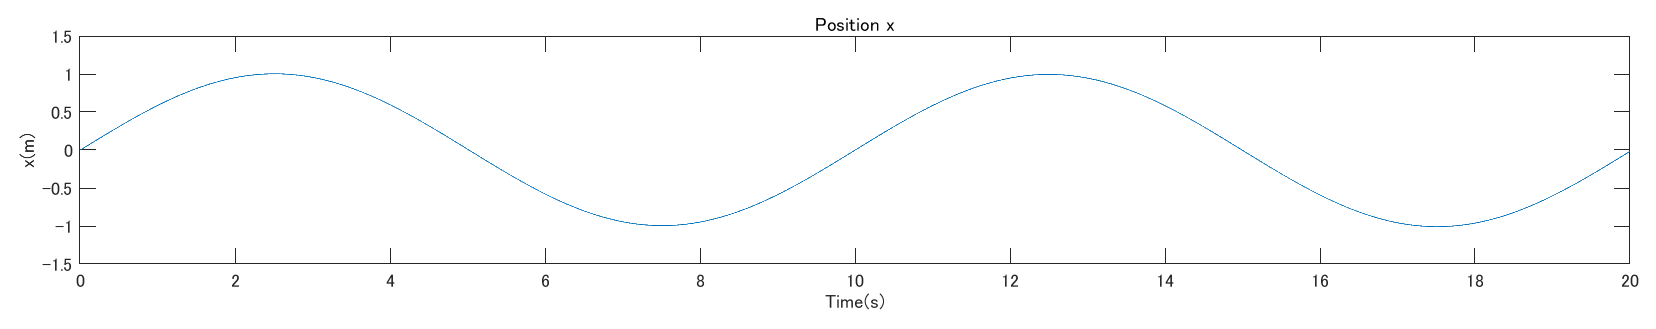
\includegraphics[width=0.6\linewidth]{R101_102_4_picture5.eps} % 拡張子付きOK(dvipdfmx前提)
\end{figure}

\begin{figure}[H] % Hで「ここに出せ」と指定(\usepackage{here}が必要)
  \centering
  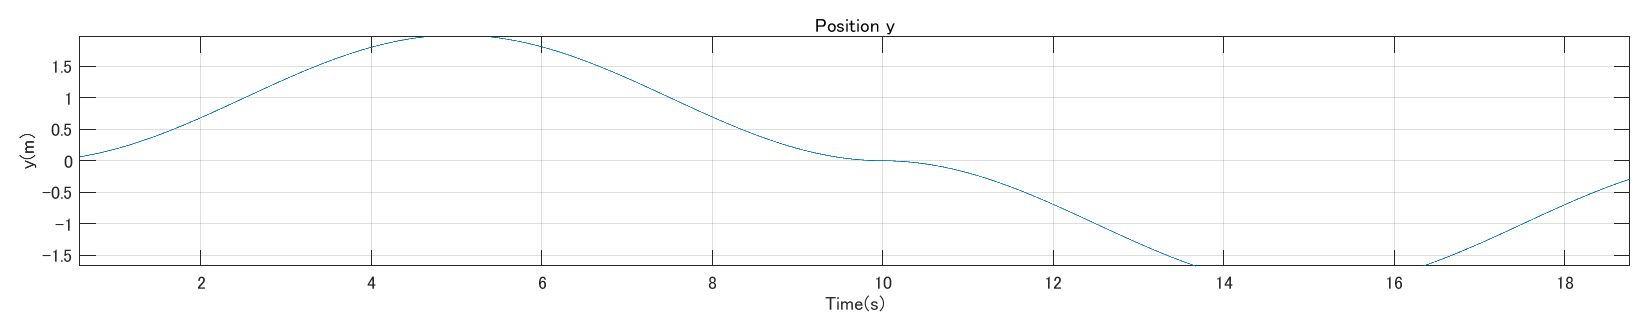
\includegraphics[width=0.6\linewidth]{R101_102_4_picture6.eps} % 拡張子付きOK(dvipdfmx前提)
\end{figure}

\begin{figure}[H] % Hで「ここに出せ」と指定(\usepackage{here}が必要)
  \centering
  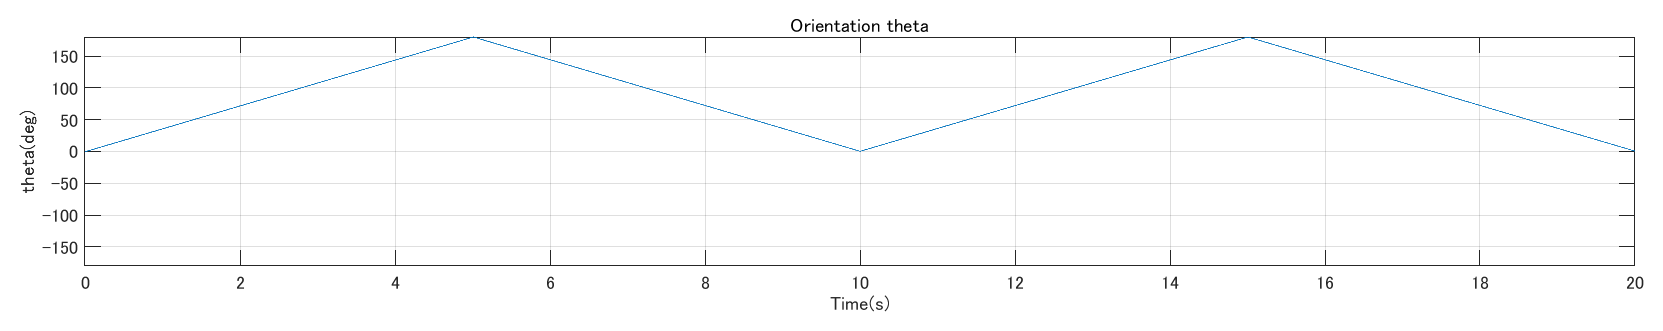
\includegraphics[width=0.6\linewidth]{R101_102_4_picture7.eps} % 拡張子付きOK(dvipdfmx前提)
\end{figure}

\begin{figure}[H] % Hで「ここに出せ」と指定(\usepackage{here}が必要)
  \centering
  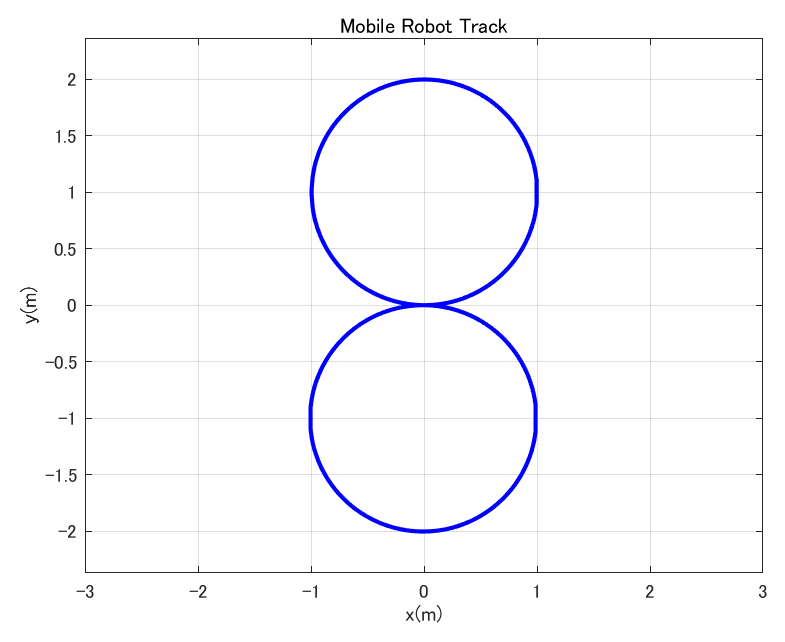
\includegraphics[width=0.6\linewidth]{R101_102_4_picture8.eps} % 拡張子付きOK(dvipdfmx前提)
\end{figure}

\chapter{参考文献}

[1] テキスト第4章まで 

[2] ChatGPT 4o

\end{document}